\documentclass[
    xcolor={svgnames,dvipsnames},
    hyperref={colorlinks, citecolor=DeepPink4, linkcolor=DarkRed, urlcolor=DarkBlue}
    ]{beamer}  % for hardcopy add 'trans'


\mode<presentation>
{
  \usetheme{Singapore}
  % or ...
  \setbeamercovered{transparent}
  % or whatever (possibly just delete it)
}

%\usefonttheme{professionalfonts}
%\usepackage[english]{babel}
% or whatever
%\usepackage[latin1]{inputenc}
% or whatever
%\usepackage{times}
%\usepackage[T1]{fontenc}
% Or whatever. Note that the encoding and the font should match. If T1
% does not look nice, try deleting the line with the fontenc.

%\usepackage{fontspec}
%\setmonofont{CMU Typewriter Text}
%\setmonofont{Consolas}

\usepackage{fontspec} 
%\usepackage[xcharter]{newtxmath}
%\setmainfont{XCharter}
\usepackage{unicode-math}
%\setmathfont{XCharter-Math.otf}
\setmonofont{DejaVu Sans Mono}[Scale=MatchLowercase] % provides unicode characters 



%%%%%%%%%%%%%%%%%%%%%% start my preamble %%%%%%%%%%%%%%%%%%%%%%

\addtobeamertemplate{navigation symbols}{}{%
    \usebeamerfont{footline}%
    \usebeamercolor[fg]{footline}%
    \hspace{1em}%
    \insertframenumber/\inserttotalframenumber
}


\usepackage{graphicx}
\usepackage{amsmath, amssymb, amsthm}
\usepackage{bbm}
\usepackage{mathrsfs}
\usepackage{xcolor}
\usepackage{fancyvrb}


% Quotes at start of chapters / sections
\usepackage{epigraph}  
%\renewcommand{\epigraphflush}{flushleft}
%\renewcommand{\sourceflush}{flushleft}
\renewcommand{\epigraphwidth}{6in}

%% Fonts

%\usepackage[T1]{fontenc}
\usepackage{mathpazo}
%\usepackage{fontspec}
%\defaultfontfeatures{Ligatures=TeX}
%\setsansfont[Scale=MatchLowercase]{DejaVu Sans}
%\setmonofont[Scale=MatchLowercase]{DejaVu Sans Mono}
%\setmathfont{Asana Math}
%\setmainfont{Optima}
%\setmathrm{Optima}
%\setboldmathrm[BoldFont={Optima ExtraBlack}]{Optima Bold}

% Some colors

\definecolor{aquamarine}{RGB}{69,139,116}
\definecolor{midnightblue}{RGB}{25,25,112}
\definecolor{darkslategrey}{RGB}{47,79,79}
\definecolor{darkorange4}{RGB}{139,90,0}
\definecolor{dogerblue}{RGB}{24,116,205}
\definecolor{blue2}{RGB}{0,0,238}
\definecolor{bg}{rgb}{0.95,0.95,0.95}
\definecolor{DarkOrange1}{RGB}{255,127,0}
\definecolor{ForestGreen}{RGB}{34,139,34}
\definecolor{DarkRed}{RGB}{139, 0, 0}
\definecolor{DarkBlue}{RGB}{0, 0, 139}
\definecolor{Blue}{RGB}{0, 0, 255}
\definecolor{Brown}{RGB}{165,42,42}


\setlength{\parskip}{1.5ex plus0.5ex minus0.5ex}

%\renewcommand{\baselinestretch}{1.05}
%\setlength{\parskip}{1.5ex plus0.5ex minus0.5ex}
%\setlength{\parindent}{0pt}

% Typesetting code
\definecolor{bg}{rgb}{0.95,0.95,0.95}
\usepackage{minted}
\setminted{mathescape, frame=lines, framesep=3mm}
\usemintedstyle{friendly}
%\newminted{python}{}
%\newminted{c}{mathescape,frame=lines,framesep=4mm,bgcolor=bg}
%\newminted{java}{mathescape,frame=lines,framesep=4mm,bgcolor=bg}
%\newminted{julia}{mathescape,frame=lines,framesep=4mm,bgcolor=bg}
%\newminted{ipython}{mathescape,frame=lines,framesep=4mm,bgcolor=bg}


\newcommand{\Fact}{\textcolor{Brown}{\bf Fact. }}
\newcommand{\Facts}{\textcolor{Brown}{\bf Facts }}
\newcommand{\keya}{\textcolor{turquois4}{\bf Key Idea. }}
\newcommand{\Factnodot}{\textcolor{Brown}{\bf Fact }}
\newcommand{\Eg}{\textcolor{ForestGreen}{Example. }}
\newcommand{\Egs}{\textcolor{ForestGreen}{Examples. }}
\newcommand{\Ex}{{\bf Ex. }}



\renewcommand{\theFancyVerbLine}{\sffamily
    \textcolor[rgb]{0.5,0.5,1.0}{\scriptsize {\arabic{FancyVerbLine}}}}

\newcommand{\navy}[1]{\textcolor{Blue}{\bf #1}}
\newcommand{\brown}[1]{\textcolor{Brown}{\sf #1}}
\newcommand{\green}[1]{\textcolor{ForestGreen}{\sf #1}}
\newcommand{\blue}[1]{\textcolor{Blue}{\sf #1}}
\newcommand{\navymth}[1]{\textcolor{Blue}{#1}}
\newcommand{\emp}[1]{\textcolor{DarkOrange1}{\bf #1}}
\newcommand{\red}[1]{\textcolor{Red}{\bf #1}}

% Symbols, redefines, etc.

\newcommand{\code}[1]{\texttt{#1}}

\newcommand{\argmax}{\operatornamewithlimits{argmax}}
\newcommand{\argmin}{\operatornamewithlimits{argmin}}

\DeclareMathOperator{\cl}{cl}
\DeclareMathOperator{\interior}{int}
\DeclareMathOperator{\Prob}{Prob}
\DeclareMathOperator{\determinant}{det}
\DeclareMathOperator{\trace}{trace}
\DeclareMathOperator{\Span}{span}
\DeclareMathOperator{\rank}{rank}
\DeclareMathOperator{\cov}{cov}
\DeclareMathOperator{\corr}{corr}
\DeclareMathOperator{\var}{var}
\DeclareMathOperator{\mse}{mse}
\DeclareMathOperator{\se}{se}
\DeclareMathOperator{\row}{row}
\DeclareMathOperator{\col}{col}
\DeclareMathOperator{\range}{rng}
\DeclareMathOperator{\dimension}{dim}
\DeclareMathOperator{\bias}{bias}


% mics short cuts and symbols
\newcommand{\st}{\ensuremath{\ \mathrm{s.t.}\ }}
\newcommand{\setntn}[2]{ \{ #1 : #2 \} }
\newcommand{\cf}[1]{ \lstinline|#1| }
\newcommand{\fore}{\therefore \quad}
\newcommand{\tod}{\stackrel { d } {\to} }
\newcommand{\toprob}{\stackrel { p } {\to} }
\newcommand{\toms}{\stackrel { ms } {\to} }
\newcommand{\eqdist}{\stackrel {\textrm{ \scriptsize{d} }} {=} }
\newcommand{\iidsim}{\stackrel {\textrm{ {\sc iid }}} {\sim} }
\newcommand{\1}{\mathbbm 1}
\newcommand{\dee}{\,{\rm d}}
\newcommand{\given}{\, | \,}
\newcommand{\la}{\langle}
\newcommand{\ra}{\rangle}

\newcommand{\boldA}{\mathbf A}
\newcommand{\boldB}{\mathbf B}
\newcommand{\boldC}{\mathbf C}
\newcommand{\boldD}{\mathbf D}
\newcommand{\boldM}{\mathbf M}
\newcommand{\boldP}{\mathbf P}
\newcommand{\boldQ}{\mathbf Q}
\newcommand{\boldI}{\mathbf I}
\newcommand{\boldX}{\mathbf X}
\newcommand{\boldY}{\mathbf Y}
\newcommand{\boldZ}{\mathbf Z}

\newcommand{\bSigmaX}{ {\boldsymbol \Sigma_{\hboldbeta}} }
\newcommand{\hbSigmaX}{ \mathbf{\hat \Sigma_{\hboldbeta}} }

\newcommand{\RR}{\mathbbm R}
\newcommand{\NN}{\mathbbm N}
\newcommand{\PP}{\mathbbm P}
\newcommand{\EE}{\mathbbm E \,}
\newcommand{\XX}{\mathbbm X}
\newcommand{\ZZ}{\mathbbm Z}
\newcommand{\QQ}{\mathbbm Q}

\newcommand{\fF}{\mathcal F}
\newcommand{\dD}{\mathcal D}
\newcommand{\lL}{\mathcal L}
\newcommand{\gG}{\mathcal G}
\newcommand{\hH}{\mathcal H}
\newcommand{\nN}{\mathcal N}
\newcommand{\pP}{\mathcal P}




\title{Modern Computational Economics \\ and Policy Applications}

\subtitle{A workshop for the IMF's Institute for Capacity Development}


\author{Chase Coleman and John Stachurski}


\date{March 2024}


\begin{document}

\begin{frame}
  \titlepage
\end{frame}







\begin{frame}
    \frametitle{Topics}

    These introductory slides provide background on modern scientific computing.

        \vspace{0.5em}
    We will discuss

    \begin{itemize}
        \item Traditional compiled languages
        \vspace{0.5em}
        \item Modern JIT compilers
        \vspace{0.5em}
        \item AI-driven scientific computing
        \vspace{0.5em}
        \item Where are we heading?
        \vspace{0.5em}
        \item Economic applications
    \end{itemize}

\end{frame}


\begin{frame}
    
    Sides, code:

    \url{https://github.com/QuantEcon/imf_2024}

\end{frame}


\begin{frame}

    Some trends: 

    \begin{figure}
       \begin{center}
        \scalebox{0.4}{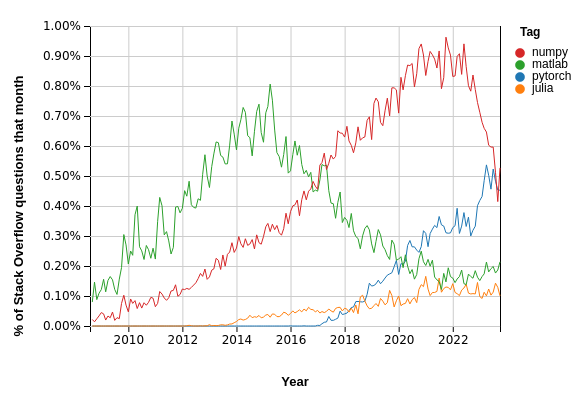
\includegraphics{pvr.png}}
       \end{center}
    \end{figure}

    Source: Stackoverflow Trends

\end{frame}


\begin{frame}

    Stack Overflow 2023 Developer Survey (50 languages)


    \begin{figure}
       \begin{center}
        \scalebox{0.5}{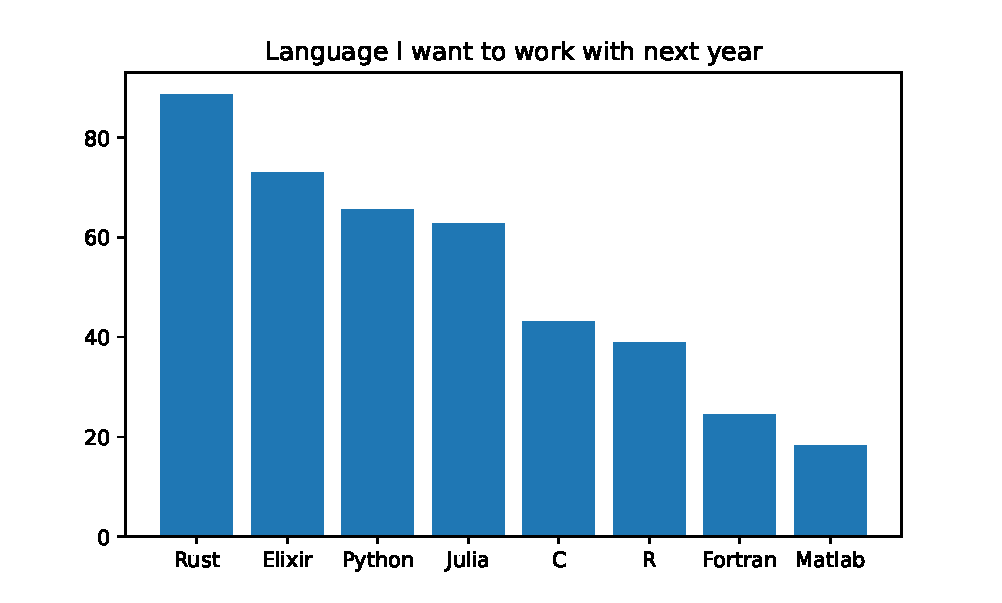
\includegraphics{admired.pdf}}
       \end{center}
    \end{figure}
    

    \hspace*{\fill}--- \url{https://survey.stackoverflow.co/2023/}


\end{frame}




\begin{frame}
    \frametitle{A review of some scientific computing environments}


    General purpose scientific computing environments:

        \vspace{0.5em}
        \vspace{0.5em}
    \begin{enumerate}
        \item Fortran / C / C++
        \vspace{0.5em}
        \vspace{0.5em}
        \item MATLAB ($\approx$ Python + NumPy)
        \vspace{0.5em}
        \vspace{0.5em}
        \item Julia ($\approx$ Python + Numba) 
        \vspace{0.5em}
        \vspace{0.5em}
        \item Python + Google JAX ($\approx$ Python + PyTorch)
    \end{enumerate}

\end{frame}



\begin{frame}
    \frametitle{Fortran / C / C++ --- static types and AOT compilers}


    \Eg Suppose we want to compute the sequence
    %
    \begin{equation*}
        k_{t+1} = s k_t^\alpha + (1 - \delta) k_t
    \end{equation*}
    %
    from some given $k_0$ 

        \vspace{0.5em}
        \vspace{0.5em}
        \vspace{0.5em}

    Let's write a function in C that 
    %
    \begin{enumerate}
        \item implements the loop 
        \vspace{0.5em}
        \item returns the last $k_t$
    \end{enumerate}


\end{frame}

\begin{frame}[fragile]
    
    \begin{minted}{c}
#include <stdio.h>
#include <math.h>

int main() {
    double k = 0.2;
    double alpha = 0.4;
    double s = 0.3;
    double delta = 0.1;
    int i;
    int n = 1000;
    for (i = 0; i < n; i++) {
        k = s * pow(k, alpha) + (1 - delta) * k;
    }
    printf("k = %f\n", k);
}
    \end{minted}

\end{frame}



\begin{frame}[fragile]
    
    \begin{minted}{zsh}
ϕ john on gz-precision …/imf_2024 on β main
❯❯ gcc solow.c -o out -lm

ϕ john on gz-precision …/imf_2024 on β main
❯❯ ./out 

x = 6.240251
    \end{minted}

\end{frame}

\begin{frame}

    Pros

    \begin{itemize}
        \item fast 
    \end{itemize}


    \vspace{0.5em}

    Cons

    \begin{itemize}
        \item time consuming to write
        \item lack of portability
        \item hard to debug
        \item hard to parallelize
        \item low interactivity
    \end{itemize}

\end{frame}

\begin{frame}[fragile]

    For comparison, the same operation in Python:
    
    \begin{minted}{python}

α = 0.4
s = 0.3
δ = 0.1
n = 1_000
k = 0.2

for i in range(n-1):
    k = s * k**α + (1 - δ) * k

print(k)

    \end{minted}

\end{frame}



\begin{frame}

    Pros

    \begin{itemize}
        \item easy to write
        \item high portability
        \item easy to debug
        \item high interactivity
    \end{itemize}

    \vspace{0.5em}

    Cons

    \begin{itemize}
        \item slow
    \end{itemize}

    \pause
    \vspace{0.5em}
    \vspace{0.5em}
    Why is pure Python slow?


\end{frame}


\begin{frame}[fragile]
    \frametitle{Problem 1: Type checking}

    Consider the Python code snippets

    \begin{minted}{python}
x, y = 1, 2
z = x + y       # z = 3
    \end{minted}

    \begin{minted}{python}
x, y = 1.0, 2.0
z = x + y       # z = 3.0
    \end{minted}

    \begin{minted}{python}
x, y = 'foo', 'bar'
z = x + y       # z = 'foobar'
    \end{minted}



\end{frame}


\begin{frame}[fragile]
    How does Python know which operation to perform?

    Answer: Python checks the type of the objects first

    \begin{minted}{python}
>> x = 1
>> type(x)
int
    \end{minted}

    \begin{minted}{python}
>> x = 'foo'
>> type(x)
str
    \end{minted}


    In a large loop, this type checking generates massive overhead
\end{frame}


\begin{frame}[fragile]
    \frametitle{Problem 2: Memory management}

    \begin{minted}{python}
>>> import sys
>>> x = [2.56, 3.21]
>>> sys.getsizeof(x) * 8      # number of bits
576                           # whaaaat???
>>> sys.getsizeof(x[0]) * 8   # number of bits
192                           # whaaaat???
    \end{minted}


    Also, lists of numbers are pointers to dispersed int/float objects ---
    not contiguous data

\end{frame}


\begin{frame}
    
    So how can we get 

    \begin{center}
    good execution speeds \navy{and} high productivity / interactivity?
    \end{center}

\end{frame}



\begin{frame}[fragile]
    \frametitle{MATLAB}

    \begin{minted}{matlab}
        A = [2.0, -1.0
             5.0, -0.5];

        b = [0.5, 1.0]';

        x = inv(A) * b
    \end{minted}


\end{frame}



\begin{frame}
    
    \begin{figure}
       \begin{center} % l b r t
        \scalebox{.6}{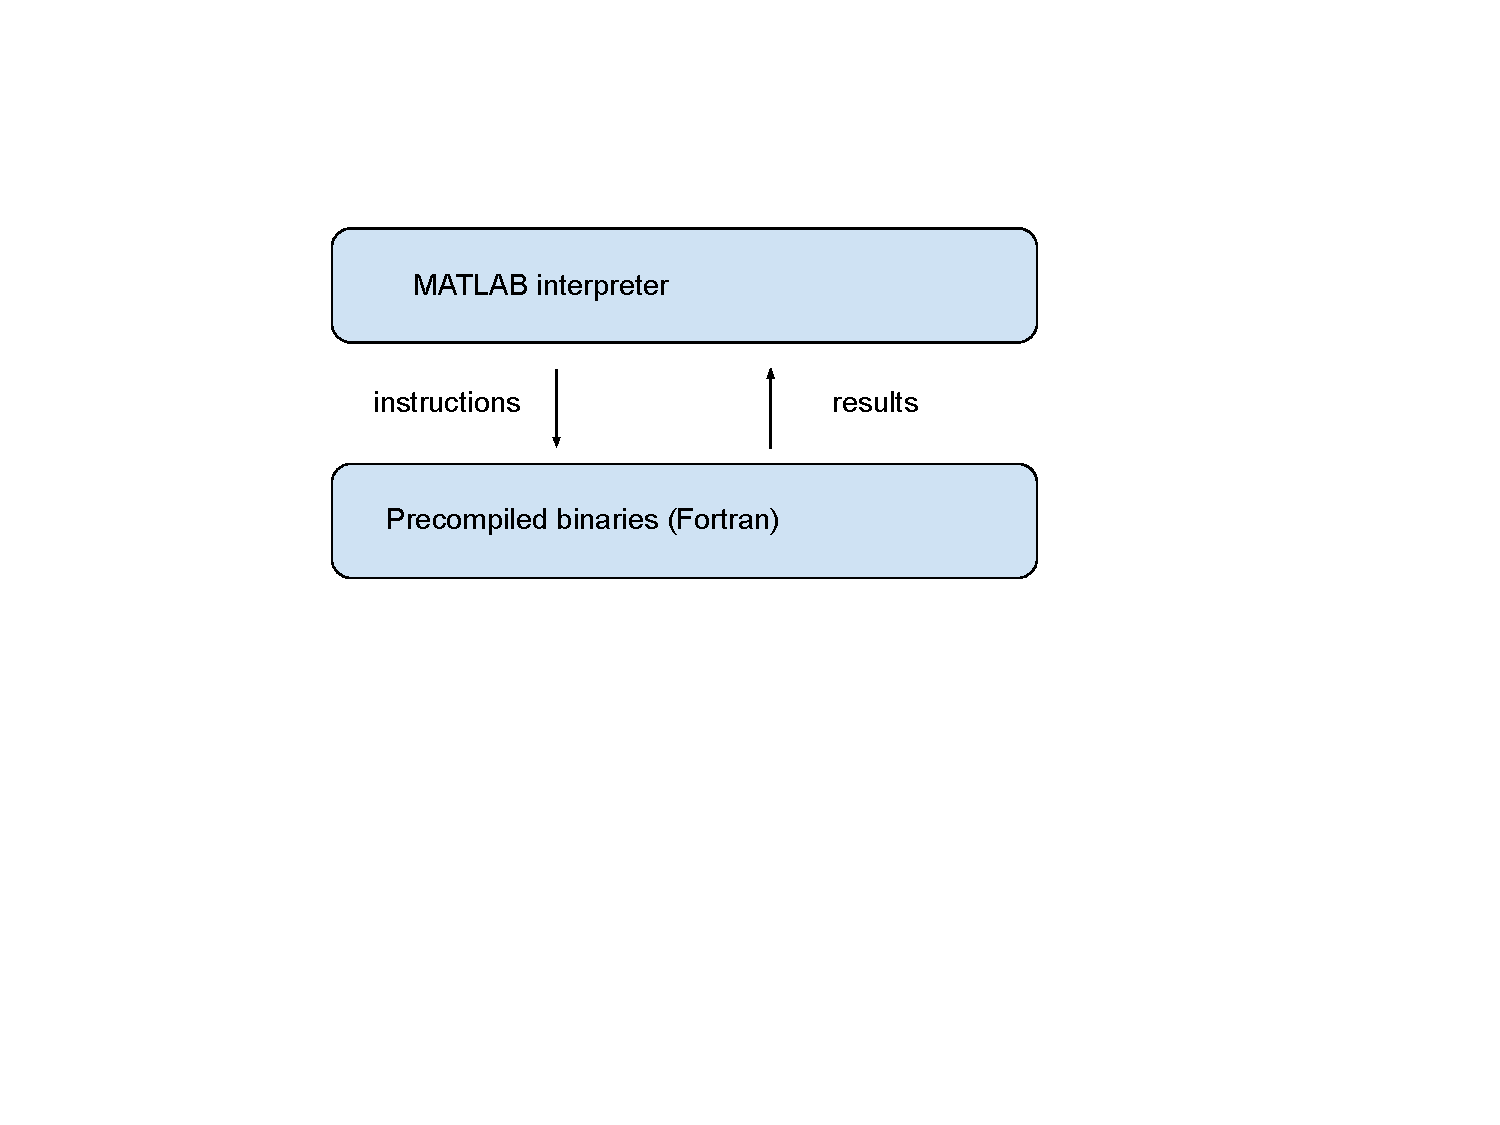
\includegraphics[trim={2cm 8cm 6cm 3cm},clip]{matlab.pdf}}
       \end{center}
    \end{figure}

    
\end{frame}


\begin{frame}[fragile]
    \frametitle{Python + NumPy}


    \begin{minted}{python}
        import numpy 

        A = ((2.0, -1.0),
             (5.0, -0.5))

        b = (0.5, 1.0)

        A, b = np.array(A), np.array(b)

        x = np.inv(A) @ b
    \end{minted}

\end{frame}

\begin{frame}

    \begin{figure}
       \begin{center} % l b r t
        \scalebox{.6}{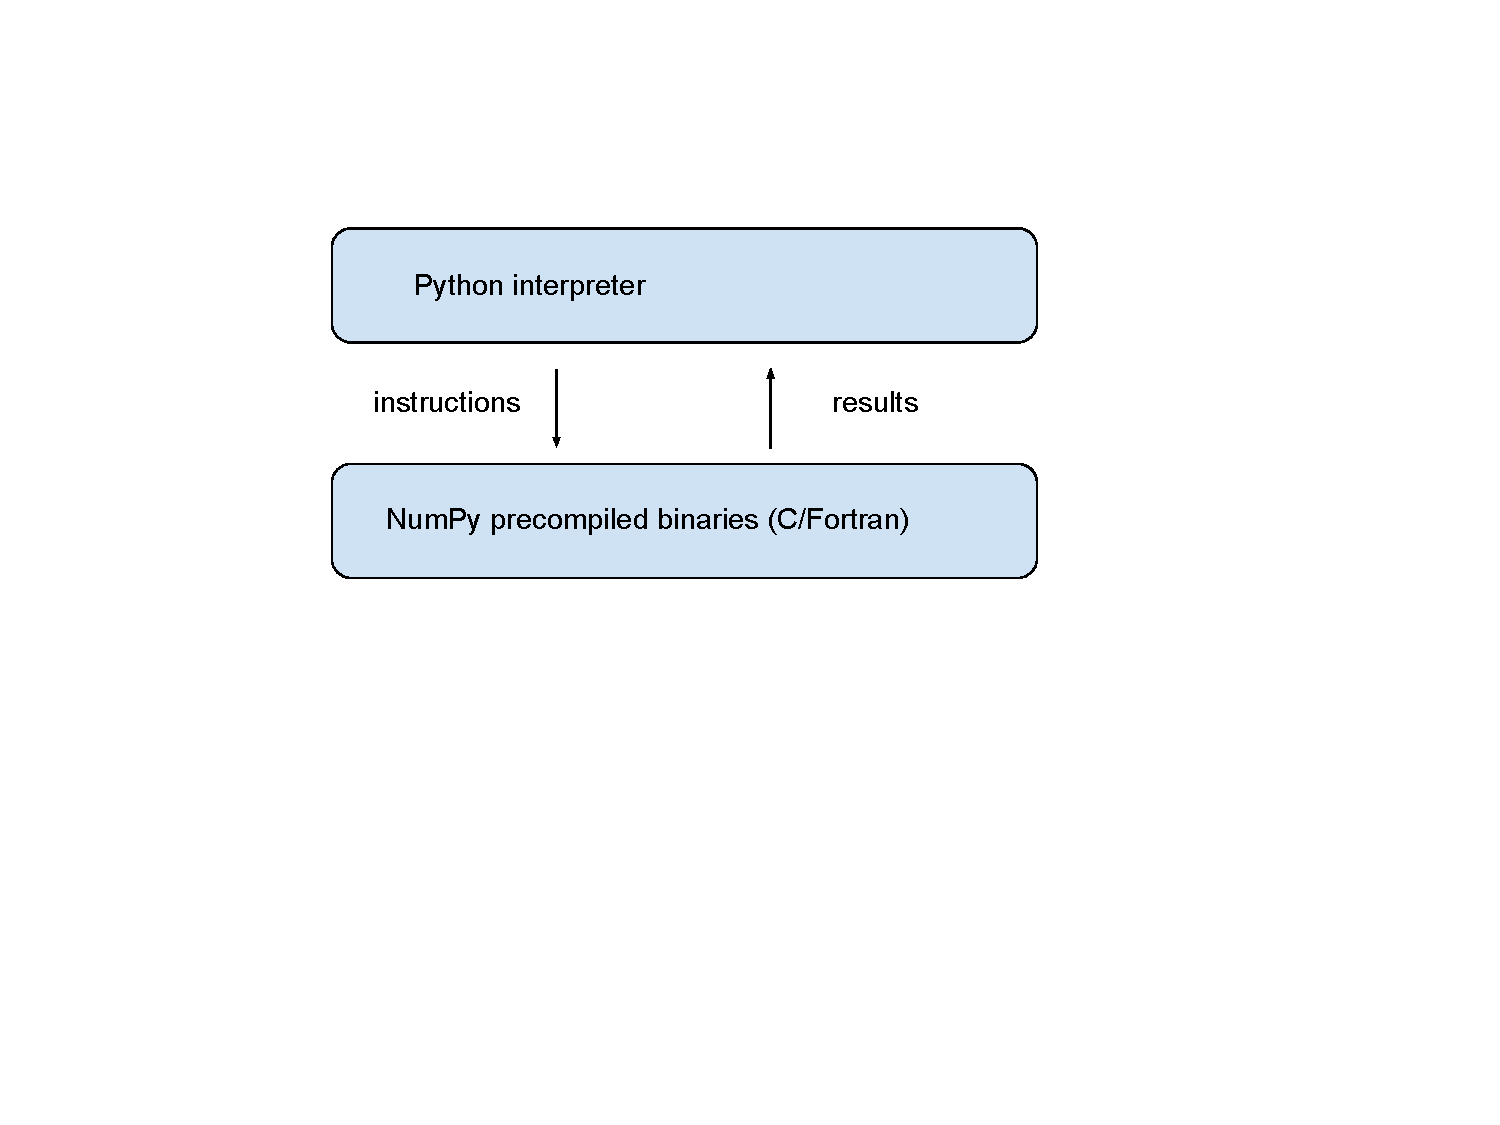
\includegraphics[trim={2cm 8cm 6cm 3cm},clip]{numpy.pdf}}
       \end{center}
    \end{figure}


\end{frame}


\begin{frame}[fragile]
    \frametitle{Julia --- rise of the JIT compilers}

    Can do MATLAB / NumPy style vectorized operations

    \begin{minted}{julia}
A = [2.0  -1.0
     5.0  -0.5]

b = [0.5  1.0]'

x = inv(A) * b
    \end{minted}
    
\end{frame}


\begin{frame}
    
    But also has fast loops via an efficient JIT compiler

    \vspace{0.5em}
    \vspace{0.5em}
    \Eg Suppose, again, that we want to compute 
    %
    \begin{equation*}
        k_{t+1} = s k_t^\alpha + (1 - \delta) k_t
    \end{equation*}
    %
    from some given $k_0$ 


    \vspace{0.5em}
    \vspace{0.5em}
    \vspace{0.5em}
    \vspace{0.5em}
    \begin{itemize}
        \item Iterative, not easily vectorized
    \end{itemize}

\end{frame}


\begin{frame}[fragile]
    
    \begin{minted}{julia}

function solow(k0, α=0.4, δ=0.1, n=1_000)
    k = k0
    for i in 1:(n-1)
        k = s * k^α + (1 - δ) * k
    end
    return k
end

solow(0.2)
    \end{minted}

    \vspace{0.5em}
    \vspace{0.5em}
    \vspace{0.5em}
    \vspace{0.5em}

    Julia accelerates \texttt{solow} at runtime via a JIT compiler

\end{frame}

\begin{frame}[fragile]
    \frametitle{Python + Numba copy Julia}
    
    \begin{minted}{python}
from numba import jit

@jit(nopython=True)
def solow(k0, α=0.4, δ=0.1, n=1_000):
    k = k0
    for i in range(n-1):
        k = s * k**α + (1 - δ) * k
    return k

solow(0.2)
    \end{minted}


    Runs at same speed as Julia / C / Fortran

\end{frame}


\begin{frame}
    \frametitle{Parallelization} 

    For tasks that can be divided across multiple ``workers,''

    \begin{equation*}
        \text{execution time = time per worker / number of workers}
    \end{equation*}

    \vspace{0.5em}
    So far we have been discussing time per worker 

    \begin{itemize}
        \item running code fast along a single thread
    \end{itemize}

    \vspace{0.5em}
    The other option for speed gains is

    \begin{itemize}
        \item divide up the execution task
    \vspace{0.5em}
        \item spread across multiple threads / processes
    \end{itemize}

\end{frame}


\begin{frame}

    Parallelization is the big game changer powering the AI revolution   


    \begin{figure}
       \begin{center}
        \scalebox{0.3}{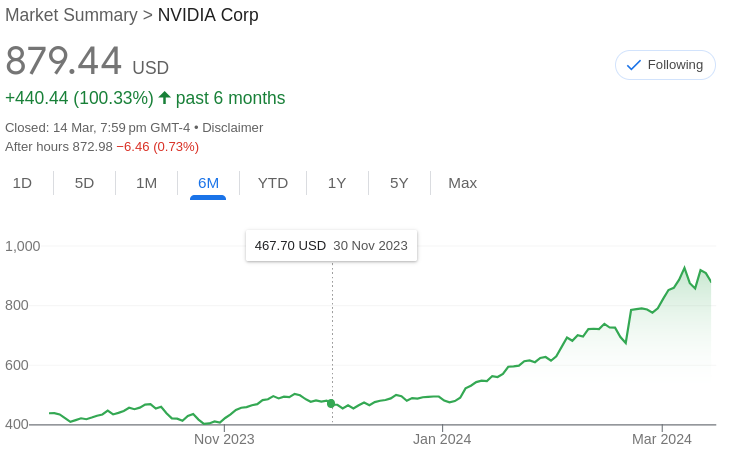
\includegraphics{nvidia.png}}
       \end{center}
    \end{figure}

\end{frame}


\begin{frame}
    
    What economists need: software that will parallelize \textbf{for us}

    \begin{itemize}
        \item automated intelligent parallelization
    \vspace{0.5em}
        \item JIT compiled
    \vspace{0.5em}
        \item portable
    \vspace{0.5em}
        \item seamlessly supports most CPUs / GPUs / hardware accelerators
    \end{itemize}



\end{frame}

\end{document}


